% !TeX root = ../../thesis.tex
\chapter{Nucleation probability assessment - a phase field methodology}\label{ch_NPA_PF_methodology}

\section{Introduction}
This chapter develops a methodology to obtain insight about the nucleation barrier from the stable shapes of particles on a planar support in 2D. The developed multi-phase phase field model is used to obtain the interface-energy-minimizing shapes and the below described \textit{domain scaling} is then used to find the shape factor of the shape. 

In order to find the equilibrium stable shape for arbitrary orientation and wetting conditions using the Moelans' multi-phase field model~\cite{Moelans2008} described also in chapter~\ref{ch_paper1}, it was necessary to implement two model extensions: volume conservation and such boundary conditions, which allow control of the interface inclination at the domain boundary. That way, the shape could be simulated in a two-phase system as long as the contact angles were known.

%The used model represents wetting of a plane by a crystal and extends the Moelans' multi-phase field model described in chapter~\ref{ch_paper1} by the following: volume conservation using the fictitious concentration field approach and the general Neumann boundary conditions to control the interface inclination at the domain boundary. 

The method to obtain the shape factors utilizes that the interface in phase field method is implicitly tracked, i.e. it evolves without any assumption on its position. Additionally, it makes use of the fact, that in the simulated geometry, the total energy of the system is in fact the total particle-liquid interface energy. Advantage of the method is that it does not a-priori assume any shape, it is thus in principle usable for non-analytic cases, where the solution is not known, e.g. a particle on a grain boundary.

The below sections first recall some fundamentals relevant for the subsequently described \textit{domain scaling} methodology. Then follows technical description of how the phase field model was extended to conserve volume and to have control over the inclination of interfaces at the domain boundary. Then, some details about the numerical implementation are included, followed by validations of the implementation in terms of how well the contact angles are reproduced for straight interface and the domain scaling methodology is then validated for circular segments with different contact angles, which is the case of heterogeneous nucleation with isotropic interface energy in 2D. The domain scaling method is then applied to the case with a particle with isotropic interface energy on top of a  grain boundary. Limitations and prospects of this approach are assessed based on the results.

%The below procedure assumes a 2D particle sitting on top of a line, the contact angles on the left and right are known. It is assumed that the environment surrounding the particle is liquid and the particle-liquid energy is anisotropic. The contact angles are determined using the Young's equation. 
%
%The following sections describe how the phase field result can be used to bring insight about the nucleation barrier using scaling of simulation domain, which is a kind of post-processing of the results. 


\section{Fundamentals}
In 2D, the Gibbs free energy difference upon a nucleus insertion in the system is due to competition between area and line energy contributions (see also Figure \ref{fig_DG_2D_sketch}). Be $A_{hom}$ the nucleus area and its interface be described by a parametric curve $\mathcal{C}$. In the isotropic case, $\mathcal{C}$ is a circle and the interfacial contribution is simply $\sigma L$, where $L=2\pi R$ is the interface length and $\sigma$ the isotropic specific interface energy. The Gibbs free energy difference of a free nucleus is then (with $\Delta G_A$ being the bulk driving force, generally speaking the supersaturation)
\begin{align}
	\Delta G_{hom} &= -\Delta G_A A_{hom} + \sigma L \\
	\label{eq_DG_hom_iso}	&= (-\Delta G_A R^2 + 2R\sigma)\pi \,,
\end{align}
which implies the critical radius
\begin{equation} \label{eq_crit_radius_2D}
	R_c = \frac{\sigma}{\Delta G_A}
\end{equation}
and critical nucleation barrier
\begin{equation} \label{eq_nucl_barr_hom_2D}
	(\Delta G_c^*)_{hom} = \hat{A}_{hom}\frac{\sigma^2}{\Delta G_A}\,,
\end{equation}
where the non-dimensional nucleus area is $\hat{A}_{hom}=A_{hom}/R^2=\pi$.

\begin{figure}
	\centering
	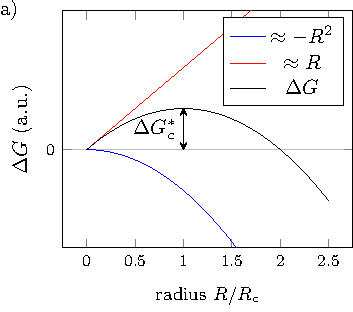
\includegraphics[width=0.5\textwidth]{DG_vs_radius_2D.pdf}
	\caption{Schematic dependence of the total energy change on the radius of the inserted nucleus in 2D.}
	\label{fig_DG_2D_sketch}
\end{figure}

In the heterogeneous nucleation, the shape factor $S(\theta)=A_{het}/A_{hom}$ scales the homogeneous total energy change upon nucleus insertion $\Delta G_{hom}$ as
\begin{equation}\label{eq_DG_het_2D}
	\Delta G_{het} = S(\theta)\Delta G_{hom} \,,
\end{equation}
which for the heterogeneous nucleation barrier implies
\begin{equation}\label{eq_nucl_barr_het_2D}
	(\Delta G_c^*)_{het} = S(\theta)(\Delta G_c^*)_{hom}\,.
\end{equation}
The nucleus radius is equal in both homogeneous and heterogeneous nucleation.

%When the interface energy is inclination-dependent $\sigma(\theta)=\sigma_0 f(\theta)$, the interface energy contribution is a line integral $\int_\mathcal{C} \sigma(\theta) \mathrm{d}l$, which can be expressed in analogy with the 3D case~[Mariaux2010] as ($X_0$ being the generalized radius of the Wulff shape with area $A_{hom}^{ani}$)
%\begin{equation}
%	\int_\mathcal{C} \sigma(\theta) \mathrm{d}l = \frac{2\sigma_0}{X_0}A_{hom}^{ani} \,,    
%\end{equation}
%which eventually allows to write the Gibbs free energy difference of a free nucleus
%\begin{equation}\label{eq_DG_hom_aniso}
%	\Delta G_{hom}^{ani} = (-\Delta G_A X_0^2 + 2\sigma_0 X_0)\hat{A}_{hom}^{ani} 
%\end{equation}
%and further its nucleation barrier
%\begin{equation} 
%	(\Delta G_c^*)_{hom} = \hat{A}_{hom}^{ani}\frac{2\sigma^2}{\Delta G_A}\,.
%\end{equation}
%In the heterogeneous anisotropic nucleation the difference in Gibbs free energy is like in equation~\eqref{eq_DG_het_2D}, having $\Delta G_{hom}^{ani}$ as in~\eqref{eq_DG_hom_aniso} and the nucleation barrier like in~\eqref{eq_nucl_barr_het_2D}, only with modified shape factor $S$ correspondingly to the Wulff shape.
%\begin{equation} \label{eq_DGcrit_het_aniso}
%	(\Delta G_c^*)_{het} = S\hat{A}_{hom}^{ani}\frac{2\sigma^2}{\Delta G_A}\,.
%\end{equation}
%For nucleation with both isotropic and anisotropic energy, the dependence of the total energy change on the particle radius has the same form~\eqref{eq_DG_hom_iso} and~\eqref{eq_DG_hom_aniso}, which is sketched in Figure~\ref{fig_DG_2D_sketch}.


\section{Methodology}
%\subsection{Principle}
%The critical nucleation barrier is the maximal possible energy change attributed to insertion a nucleus of a particular shape, interface energy and in the present supersaturation (bulk driving force in general). 
The simulated system geometry is sketched in Figure~\ref{fig_sketch_domain_scaling_PF}. A two-phase system of a particle in a liquid was described by two phase field variables in Moelans' model, one representing the liquid parent phase ($\eta_1$) and the second ($\eta_2$) representing the particle (possibly with anisotropic interface energy). The bottom domain boundary then represents the substrate and the interface inclination $\vartheta_L,\vartheta_R$ in the two contact points is controlled by the boundary condition as indicated in the figure.
\begin{figure}
	\centering
	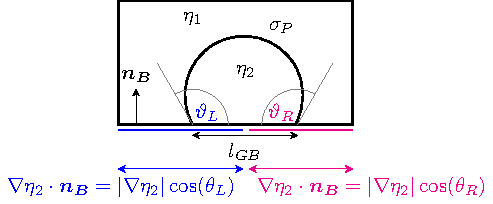
\includegraphics[width=0.8\textwidth]{sketch_geometry_PF_NPA.pdf}
	\caption{Sketch of the geometry in the phase-filed simulations used in the domain scaling methodology for nucleation barrier assessment. The symbols $\vartheta_L,\vartheta_R$ denote tangent angles in the contact points and $\theta_L,\theta_R$ the normal ones. The two intervals on the bottom domain boundary with the different interface inclination imposed are indicated  by blue color on the left half of the domain and by magenta on the right one (note that $\eta_1$ has analogous boundary conditions which must be consistent). $l_{GB}$ is the length of the grain boundary interval between the contact points. $\sigma_P$ is the particle-liquid interface energy.}
	\label{fig_sketch_domain_scaling_PF}
\end{figure}

Volume conservation was assured using the fictitious concentration field described in the section~\ref{sec_volume_cons_PF_ch_NPA_PF}. 

The particle-liquid interface energy $\sigma_P$ was assumed, together with the contact angles $\vartheta_L, \vartheta_R$ between the solid-liquid interface and the bottom domain boundary. How these angles were imposed is described in section~\ref{sec_general_NBC_ch_NPA_PF}.

The domain scaling methodology is in fact a post-processing of the result of phase field simulation. By the result, it is meant the phase fields corresponding to the liquid and to the particle within the simulation grid. Then, the grid spacing $\Delta x$ is scaled and the model parameters are re-computed accordingly. The particle area fraction $\xi=A_P/A_D$ in the scaled system remains the same, but its area $A_P$ and perimeter are scaled accordingly. Using the (unchanged) phase fields and re-computed parameters, the total interface energy is re-evaluated by the free energy functional for the new scale. The domain scaling is sketched in Figure~\ref{fig_domain_scaling}a. 

\begin{figure}
	\centering
	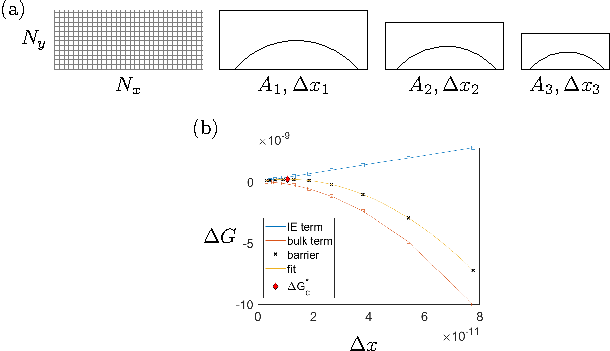
\includegraphics[width=0.7\textwidth]{combined_sketch_domain_scaling.pdf}
	\caption{Nucleation barrier determination using domain scaling. In (a) sketch of domain scaling. The area fraction of the particle is preserved, as well as the number of grid points $N_x, N_y$. $A_i$ are scaled areas of the domain and $\Delta x_i$ is the i-th scaled grid spacing in meters. In (b) the energy contributions were plotted for each $\Delta x_i$, the barrier being denoted by black crosses and the critical nucleation barrier determined by fitting of parabolic function is indicated by red diamond.}
	\label{fig_domain_scaling}
\end{figure}	

Note that the free energy functional only accounts for the solid-liquid interface energy, but in the total energy change, there must be included also the term representing the replacement of the former planar substrate-liquid interface with specific energy $\sigma_S$ by the grain boundary: $l_{GB}(\sigma_{GB}-\sigma_S)$. Because the Young's equation for triple junctions of isotropic interfaces reads
\begin{equation}\label{eq_young_iso}
	\sigma_S = \sigma_{GB}+\sigma_P\cos(\vartheta) \,,
\end{equation}
the grain-boundary-energy term can be thus re-written as $-l_{GB}\sigma_P\cos(\vartheta)$, which allows us to disregard the values of the substrate and grain boundary energy. In the phase field simulation, the distance between the contact points is interpreted as $l_{GB}$ (see Figure~\ref{fig_sketch_domain_scaling_PF}) and the above term is added to the total interface energy change upon the nucleus insertion $\Delta G_\sigma$, hence when denoting the free energy functional as $F(\eta,\nabla\eta)$ it can be written
\begin{equation}
	\Delta G_\sigma = F(\eta,\nabla\eta) - l_{GB}\sigma_P\cos(\vartheta) \,.
\end{equation}
Note that $l_{GB}$ is necessarily scaled as well during the domain scaling procedure.

The above procedure provided the total interface energy change upon the particle insertion as function of the length scale ($\Delta x_i$ in Figure~\ref{fig_domain_scaling}a). Even though it is not the particle radius as in~\eqref{eq_DG_hom_iso}, the same physical dimension (length) of the grid spacing assures that the order of the polynomial $\Delta G(\Delta x) = a(\Delta x) - b(\Delta x)^2$ is the same as in~\eqref{eq_DG_hom_iso}.

When the driving force $\Delta G_A$ is explicitly assumed, the bulk energy contribution can be computed using each of the absolute values of the scaled particle area $A_P$. Because the interface energy contribution was already computed for each scaled system, it is possible to subtract the two to obtain the total energy change in insertion of those particles, as is shown in Figure~\ref{fig_domain_scaling}b. For illustration, multiple scaling steps were taken here, but with the simple parabolic dependence of $\Delta G$ in 2D, only 3 points would suffice to unambiguously determine its parameters. Finding the position of the maximum is then trivial. 

The maximum parabola value is the critical nucleation barrier $(\Delta G^*)_{het}$ for the investigated heterogeneous equilibrium shape. However, a more practical quantity is the corresponding shape factor $S$, which can be then obtained from equations~\eqref{eq_nucl_barr_hom_2D} and~\eqref{eq_nucl_barr_het_2D} as
\begin{equation} \label{eq_NPA_PF_formula}
	S = (\Delta G_c^*)_{het}\frac{\Delta G_A}{\hat{A}_{hom}\sigma_0^2} \,.
\end{equation}
Note, that one needs to know the non-dimensional area of the isolated equilibrium shape $\hat{A}_{hom}=A_{hom}/R^2$. Essentially, that is an area of the isolated Wulff shape of unit radius (in this study it was obtained numerically from Wulff shapes plotted with fine resolution).

Recall, that the contact angles of the particle with the substrate were the input to the phase field simulation, hence the obtained shape factor $S$ is a function of the particular assumed conditions. 

The domain scaling procedure does not depend on whether the interface energy was isotropic or anisotropic, because the used formulas leading to~\eqref{eq_NPA_PF_formula} are equal in the two cases~\cite{Mariaux2011}. Only in the case with inclination-dependent interface energy more steps are required in evaluation of the free energy functional $F(\eta,\nabla\eta)$ because the formulas for model parameters are more complicated than in the isotropic case.

\section{Model}
Because the Moelans' model with anisotropic interfaces was already extensively introduced in section~\ref{sec_Models}, this section covers only the necessary extensions to simulate the system as sketched in Figure~\ref{fig_sketch_domain_scaling_PF}, 

	\subsection{General Neumann boundary conditions to control interface inclination at domain boundary}\label{sec_general_NBC_ch_NPA_PF}
	This model extension was inspired by~\cite{Granasy2007}. It allows to control the interface inclination angle $\phi$ at the boundary, which thus becomes an input parameter. The principle is explained using a single phase field $\eta(\bm{r})$. 
	First, we remark that the standard Neumann boundary conditions $\nabla\eta\cdot\bm{n_D}=0$ must be a special case of the general Neumann boundary conditions ($\bm{n_D}$ is the domain boundary normal). The regular Neumann boundary condition implies perpendicularity of the phase field gradient to the domain boundary normal. In other words, the interface is perpendicular to the domain boundary. Generally, we can write $\bm{n_D}\cdot \nabla\eta=|\nabla\eta|\cos(\phi)$. In the model by Granasy~\cite{Granasy2007}, the local magnitude of phase field gradient may be expressed using the local phase field value, giving rise to expression of the boundary condition as
	\begin{equation}
		\bm{n_D}\cdot \nabla\eta=\frac{\cos(\phi)}{\delta\sqrt{2}}\eta(1-\eta)\,,
	\end{equation}
	where $\delta$ is the interface width. At the domain boundary, the gradient $\nabla\eta$ is expressed as a polynomial, which allows straightforward implementation of the condition, especially in rectangular simulation domains.\\
	
	In Moelan's model, the interface normal between the phase fields $\eta_i,\,\eta_j$ denoted $\bm{n}_{i,j}$ is defined as local difference in neighboring phase field gradients (see equation~\ref{eq_def_inclination}). In the spirit of the introductory example we can write
	\begin{equation}
		\bm{n_D}\cdot\bm{n}_{i,j} = \cos(\phi) \quad \implies \quad \bm{n}\cdot(\nabla\eta_i-\nabla\eta_j) = |\nabla\eta_i-\nabla\eta_j|\cos(\phi) \,.
	\end{equation}
	Now we have single boundary condition with the correct physical interpretation (fixed inclination angle at the boundary) but because the governing equations are solved for the phase fields, a set of equivalent boundary conditions (one for each phase field) must be derivable from the above. In these independent boundary conditions, it must be possible to express the gradient magnitude (the introductory example finds a polynomial of local phase field values equal to the gradient magnitude). \\
	The first problem (i.e. coupling in the boundary conditions) would be solved if one gradient could be written as a function of the other and vice versa. However, this dependence is non-analytical for all $\gamma_{i,j}\neq1.5$. For $\gamma_{i,j}=1.5$ it is simply $\eta_i = 1-\eta_j$ and therefore also $\nabla\eta_i=-\nabla\eta_j$.~\cite{Moelans2008} \\
	The second problem (i.e. the expression for gradient magnitude) is also enabled by the choice $\gamma=1.5$, as in such case there were derived analytic expressions for the gradients $\nabla\eta_i,\nabla\eta_j$~\cite{Moelans2008}. In 1D system with 2 phase fields holds
	\begin{equation} \label{eq_PFgradient_analytic}
		\begin{split}
			\frac{\mathrm{d}\eta_i}{\mathrm{d}x} &= \sqrt{\frac{2m}{\kappa_{i,j}}}\eta_i(1-\eta_i) \overset{\mathrm{2D, 3D}}{=} |\nabla\eta_i| \\
			\frac{\mathrm{d}\eta_j}{\mathrm{d}x} &= \sqrt{\frac{2m}{\kappa_{i,j}}}\eta_j(1-\eta_j) \overset{\mathrm{2D, 3D}}{=} |\nabla\eta_j| \,.
		\end{split}
	\end{equation}
	Validity of the last equation sign in 2D and 3D (in systems with 2 phase fields) can be checked using the expressions in~\cite{Moelans2008} as follows. Write the equation 7 from~\cite{Moelans2008} for 2D. From it one gets 2D equivalents of equations 8a and 8b, where $\frac{\mathrm{d}\eta}{\mathrm{d}x}$ is replaced by $|\nabla\eta|$. Further, because the equation 19 does not depend on problem dimensionality, we obtain here the expressions in equation~\ref{eq_PFgradient_analytic}. In systems with more than two phase fields, the general expression for the gradient magnitude is more complex. However, the same relations are satisfied at a pair-wise interface not close to the triple junction. \\
	With the above and assuming that there is no triple junction near the domain boundary, we can thus write
	\begin{equation}
		\begin{split}
			\bm{n}\cdot(\nabla\eta_i-\nabla\eta_j) &= 2\bm{n}\cdot\nabla\eta_i = 2|\nabla\eta_i|\cos(\phi) \\ &= -2\bm{n}\cdot\nabla\eta_j = -2|\nabla\eta_j|\cos(\phi) \,,
		\end{split}
	\end{equation}
	which provides very similar BC like in the introductory example for each of the two phase fields.\\
	The only way how to use these relations is to have $\gamma_{i,j}=1.5$. In the case of inclination-dependent interface energy $\sigma_{i,j}(\theta_{i,j})=\sigma_{i,j}^0h_{i,j}^\sigma(\theta_{i,j})$, it is necessary to express the anisotropy fully by the parameter $\kappa_{i,j}(\theta_{i,j})$, i.e. to use the IWvK model.
	
	\subsection{Volume conserving multi phase field models}\label{sec_volume_cons_PF_ch_NPA_PF}
	There are several approaches which accomplish the volume conservation of some species or phases. Each has its drawbacks though. It was not clear which of the possible approaches was the most convenient for coupling with inclination-dependent interface energy in curvature-driven systems.
	
	Three conceptually different solutions can be used in a multi-phase field model, which are known to the author: Cahn-Hilliard equation, Lagrange multipliers and fictitious concentrations field. 
	
	Given the intended application with anisotropic interface energy and the complicated driving force, a less computationally demanding option than the Cahn-Hilliard equation was seeked, because that one is a partial differential equation of 4-th order in space. 
	
	The approach using Lagrange multipliers to conserve volume was thoroughly considered, but eventually it was found out that in Moelan's model is not a suitable solution. The reason is that the volume of a single phase/grain is defined using all other phase fields, which introduces excessive computational complexity in application of the principles leading to volume conservation. All related details and explanations can be found in Appendix~\ref{ch_lagrange_multipliers_PF}.
	
	The approach using fictitious concentration field was eventually assessed as the most convenient one. It is not new in combination with Moelans' multi-phase field model (see e.g.~\cite{Yadav2016,Yadav2018vol_cons}). It is briefly reviewed in the following subsection. 
		
		\subsubsection{Fictitious concentration field}
		The idea in the fictitious concentration field approach to conserve volume of a phase field is to couple the Allen-Cahn equation to a conserved concentration field in such a way, that the change in phase fraction is only possible with exchange of species between phases. If the concentration of the independent species is set to equilibrium value and the energy valley is steep enough, no phase transformation occurs and the volume of the phase fraction should be conserved through the system. 
		
		In the description below, it is assumed that there are two phases, one solid and the other liquid.
		
		The free energy functional is then
		\begin{equation}
			F_{cons} = \int_V \left[ f_{hom}(\vec{\eta},\nabla\vec{\eta},c) + f_{grad}(\vec{\eta},\nabla\vec{\eta}) \right] \mathrm{d}V \,,
		\end{equation}
		with   
		\begin{align}
			f_{hom}(\vec{\eta},\nabla\vec{\eta},c)  &= f_0(\vec{\eta},\nabla\vec{\eta}) + f_{chem}(\vec{\eta},c) \\
			f_{chem}(\vec{\eta},c) &= h_S(\vec{\eta})f_S(c) + h_L(\vec{\eta})f_L(c)
		\end{align}
		$h_S(\vec{\eta}), h_L(\vec{\eta})$ are solid and liquid interpolation functions. Assuming that the solid phase is composed of $s$ phase fields $\eta_{S1},\eta_{S2},\dots,\eta_{Ss}$ and the liquid phase of $l$ phase fields $\eta_{L1},\eta_{L2},\dots,\eta_{Ll}$ we can write
		\begin{align}
			h_S(\vec{\eta}) &= \frac{\sum_i^s \eta_{Si}^2}{\sum_i^s \eta_{Si}^2 + \sum_j^l \eta_{Lj}^2}   \\
			h_L(\vec{\eta}) &= \frac{\sum_j^l \eta_{Lj}^2}{\sum_i^s \eta_{Si}^2 + \sum_j^l \eta_{Lj}^2} \quad .
		\end{align}
		Parabolic energy approximation will be used for the concentration dependence of the homogeneous phase free energy densities $f_S(c), f_L(c)$ as
		\begin{align}
			f_S(c_S) &= A(c_S-c_{S,eq})^2 \\
			f_L(c_L) &= B(c_L-c_{L,eq})^2 \,.
		\end{align}
		An ideal solution approximation was adopted.
		
		The governing equations for two phase fields are then
		\begin{align}
			\frac{\partial \eta_1}{\partial t} &= -L\left[\frac{\partial f_0}{\partial \eta_1} - \nabla\cdot \frac{\partial F}{\partial (\nabla\eta_1)} + \frac{\partial h_S}{\partial \eta_1}[f_S(c_S) - f_L(c_L) - (c_S-c_L)\mu] \right] \\
			\frac{\partial \eta_2}{\partial t} &= -L\left[\frac{\partial f_0}{\partial \eta_2} - \nabla\cdot \frac{\partial F}{\partial (\nabla\eta_2)} + \frac{\partial h_S}{\partial \eta_2}[f_S(c_S) - f_L(c_L) - (c_S-c_L)\mu] \right] \\
			\mu &= 2A(c_L-c_{L,eq})\\
			\frac{\partial c}{\partial t} &= \frac{D}{A}\Delta\mu  = 2D\Delta(c_L-c_{L,eq})
		\end{align}
		where the diffusion coefficient $D$ is a constant.
		
		The interpolation functions have the following property
		\begin{equation}
			\frac{\partial h_S}{\partial \eta_p} = -\frac{\partial h_L}{\partial \eta_p}
		\end{equation}
		
		%The difference in grand potential in the solid and liquid phase is the driving force for change of the phase fraction. It is assumed that $A=B$ and thus
		%\begin{equation}
		%	f_S(c_S) - f_L(c_L) - (c_S-c_L)\mu = 
		%\end{equation}

\section{Numerical implementation}
The simulations were carried out using the same MATLAB programme, which was used in the previous chapter~\ref{ch_paper1}, hence only some extra considerations are commented here.

The Appendix~\ref{ch_numerical_implementation} contains the necessary modifications to the finite-difference algorithm when implementing the general Neumann boundary conditions. Eventually, the changes affected all the finite difference operators (standing in place of unidirectional or mixed derivatives and laplacian), but only in the parts of the matrices, which involve the nodes at the domain boundary.

The parameters of the phase field simulations needed to reproduce the results are in Table~\ref{tab_parameters_PF_NPA}. Regarding the volume conservation, it was validated that with the listed parameters, the area of the conserved field would change no more than about 1~\% from its initial value in practical simulations, which is sufficient for the equilibrium shape simulations and subsequent barrier determination.

\begin{table}[]
	\centering
	\caption{Parameters in the phase field simulation (unless stated otherwise). The parameters in the top part correspond to the Moelans' model, in the bottom one to the diffusion equation used in the fictitious concentration field approach to conserve volume of the simulated particle. The not mentioned parameters $m,\kappa, L$ in Moelans' model can be determined using the dedicated published MATLAB functions~\cite{Minar2022dataset}.}
	\begin{tabular}{c|c|c|c}
		symbol & parameter & units & values  \\ \hline
		$l_{IW}$ & interface width & \unit{\m} & \qty{1e-9}{}\\ 
		$\sigma_P$ & particle-liquid isotropic interface energy & \unit{\J/\m^2} & 1 \\
		$\Delta x$ & grid spacing & \unit{\m} & $l_{IW}/7$\\
		$C$	& Courant number	&	- & 0.18 \\
		$\mu_{P}$	& particle-liquid interface mobility	&	\unit{\m^4/\J\s} & \qty{7.5e-16}{} \\
		$\Delta t$	& time step	&	\unit{\s} & using~\eqref{eq_Courant_nr} \\
\hline	$A$ & steepness of parabolas & \unit{\J/\m^3} & \qty{3.1623e-11}{} \\
		$D$ & diffusion coefficient & \unit{\m^2/\s} & $0.3\Delta x^2/\Delta t$ \\
		$c_{L,eq}$ & equilibrium molar fraction in liquid & - & 0.02 \\
		$c_{S,eq}$ & equilibrium molar fraction in solid & - & 0.98 \\
		$M$ & diffusion coefficient in C-H equation & \unit{\m^5/\J\s} & $M=D/A$
	\end{tabular}
	\label{tab_parameters_PF_NPA}
\end{table}

The re-computation of the model parameters during the domain scaling was carried out using the same MATLAB functions~\cite{Minar2022dataset} as used in chapter~\ref{ch_paper1} and~\cite{Minar2022}.


\section{Validations}
	\subsection{Tilted straight line}
	The implementation of general Neumann boundary conditions controlling the inclination angle at the domain boundary was validated in simulations sketched in Figure~\ref{fig_sketch_tilted_plane_validation}. Note that the volume was not conserved in these simulations. A slightly different approach had to be taken in the case with isotropic and anisotropic interface energy, as described below.
	
	In the case with isotropic interface energy, the initial condition for the simulation was a tilted line, which was inclined under different angle $\vartheta_{init}$ than the imposed inclination angle $\vartheta$. The simulation ran until the total energy converged (i.e. until the change in energy per time step was smaller than a threshold). The final state was expected to be a line aligned under the target angle $\vartheta$. From linear fit of the final phase field contour, the resulting inclination angle was read out. A range of angles between 15\textdegree-165\textdegree was probed, and the results were plotted in Figure~\ref{fig_tilted_plane_validation_results}a. As can be seen, a perfect match was achieved.
	
	When validating the same with inclination-dependent interface energy, the methodology had to be modified slightly: the straight line was placed in its imposed position already in the initial condition, i.e. $\vartheta_{init}=\vartheta$. That was because once any curvature appeared in the straight line (which happened when the interface was forced to move by the boundary conditions), it began deforming and there remained no straight line. To assure that the tilted line be the equilibrium state of the system, the anisotropy function was always rotated so that the target inclination angle $\vartheta$ corresponded to the minimal interface energy. Only then the straight line could be immobile and the general Neumann BC could be validated in the same way like with the isotropic interface energy, i.e. simulation until energy convergence and linear fit of the contour. The target angle was observed very accurately in this case as well, as can be seen in Figure~\ref{fig_tilted_plane_validation_results}b.
	\begin{figure}
		\centering
		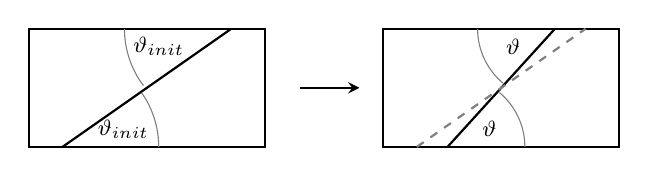
\begin{tikzpicture}[scale=1.5]
			\draw[thick] (0,0) rectangle (2,1);
			\draw[thick] (1-0.5/0.7,0) -- (1+0.5/0.7,1);
			\draw (0.8,0.15) node {\footnotesize$\vartheta_{init}$};
			\draw (1.1,0.85) node {\footnotesize$\vartheta_{init}$};
			\draw[gray] (0.81,1) arc (180:217:0.8);
			\draw[gray] (1.1,0) arc (0:35:0.8);
			
			\draw[thick,-stealth] (2.3,0.5) -- (2.8,0.5);
			
			\draw[thick] (3,0) rectangle (5,1);
			\draw[thick] (4-0.5/1.1,0) -- (4+0.5/1.1,1);
			\draw[dashed,gray,thick] (4-0.5/0.7,0) -- (4+0.5/0.7,1);
			\draw (3.9,0.15) node {\footnotesize$\vartheta$};
			\draw (4.1,0.85) node {\footnotesize$\vartheta$};
			\draw[gray] (3.8,1) arc (180:230:0.6);
			\draw[gray] (4.2,0) arc (0:50:0.6);
		\end{tikzpicture}
		\caption{Validation of the general NBC for control of the inclination angle at the boundary - tilted line simulations (isotropic interface energy). In the simulations with inclination-dependent interface energy there was $\vartheta_{init}=\vartheta$}
		\label{fig_sketch_tilted_plane_validation}
	\end{figure}
	\begin{figure}
		\centering
		\begin{tikzpicture}
			\node[below right, inner sep=0] (L) at (0,0) {
				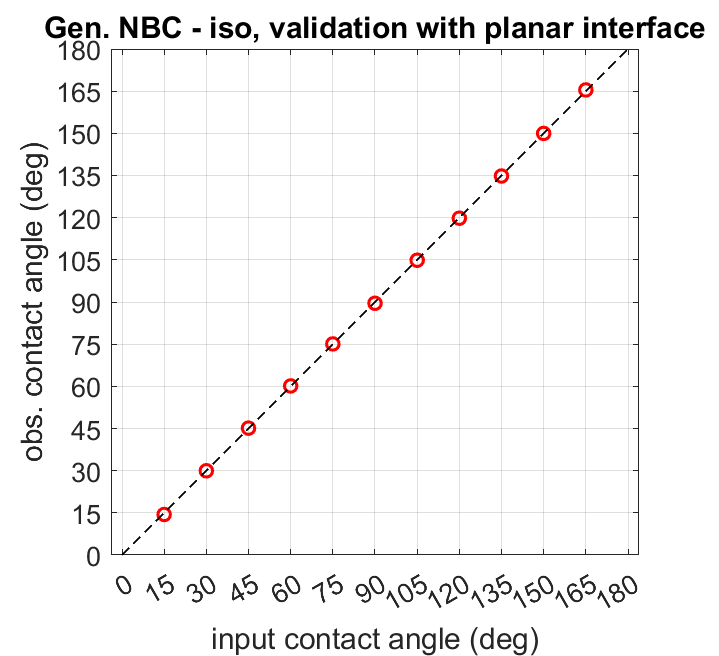
\includegraphics[width=0.48\textwidth]{validation_iso_specBC_planar.png}};
			\node[below right, inner sep=0] (R) at (L.north east) {
				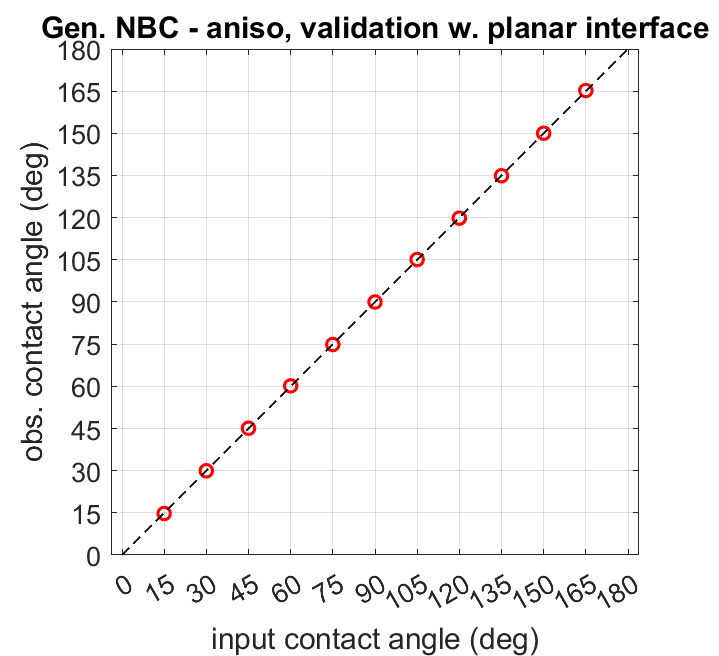
\includegraphics[width=0.48\textwidth]{validation_aniso_specBC_planar_final.png}};
				
			\draw[above ] (L.north west) node {(a)};
			\draw[above ] (R.north west) node {(b)};
		\end{tikzpicture}
		\caption{Results of tilted plane validation. In a) the result with isotropic interface, in b) with anisotropic one. }
		\label{fig_tilted_plane_validation_results}
	\end{figure}
		
\section{Results}
First, the methodology is used to determine the shape factor in isotropic heterogeneous nucleation as a proof-of-concept application.


\subsection{Particle on a plane (isotropic interface energy)}
In heterogeneous nucleation with isotropic interface energy in 2D, the equilibrium shape is a circular segment and the shape factor as function of the tangent contact angle (wetting angle) $\vartheta$ (see Figure~\ref{fig_sketch_domain_scaling_PF}) is
\begin{equation}
	S(\vartheta) = \frac{2\vartheta - \sin(2\vartheta)}{2\pi} \,.
\end{equation}
A series of phase field simulations was run in the geometry as in Figure~\ref{fig_sketch_domain_scaling_PF} with $\vartheta_L=\vartheta_R$ to assess the above dependence of shape factor on the wetting angle. See Table~\ref{tab_PF_NPA_param_particle_onplane} for details on the simulation grid in the respective simulations.
\begin{table}
	\centering
	\caption{Simulation grid dimensions in individual simulations of a particle with isotropic interface energy on a plane in 2D. The grid aspect ratio was determined based on the expected shape aspect ratio.}
	\label{tab_PF_NPA_param_particle_onplane}
	\begin{tabular}{c|c}
		$\vartheta$ & $N_x\times N_y$ \\ \hline
	 	15	&	$546\times 42$	\\
	 	30	&	$382\times 51$	\\
	 	45	&	$308\times 64$	\\
	 	60	&	$261\times 75$	\\
	 	75	&	$226\times 87$	\\
	 	90	&	$198\times 99$	\\
	 	105	&	$176\times 111$	\\
	 	120	&	$162\times 121$	\\
	 	135	&	$152\times 129$	\\
	 	150	&	$145\times 135$	\\
	 	165	&	$141\times 139$	
	\end{tabular}
\end{table}
It is assumed, that the obtained shape is the equilibrium one, which is assured by conditional stopping of the simulation, when the total interface energy converged (i.e. its change in the new time step was below threshold). 

The contact angles were the same as in the tilted plane validation, i.e. from $\vartheta=15$\textdegree~to $\vartheta=165$\textdegree~with a 15\textdegree~step. The initial condition corresponded to the target circle segments to reduce the computation time. Using the equation~\eqref{eq_NPA_PF_formula} and taking into account that the non-dimensional area for a circle is $\hat{A}_{circle}=\pi$, the results in Figure~\ref{fig_result_NPA_PF_S_iso} were obtained.
\begin{figure}
	\centering
	\begin{tikzpicture}
		\draw node (1) at (0,0) {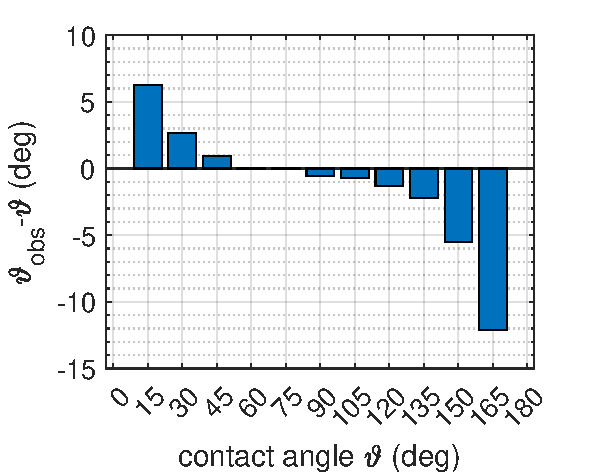
\includegraphics[width=0.49\textwidth]{NPA_PF_abserr_iso.pdf}};
		\draw node[below right] (2) at (1.north east) {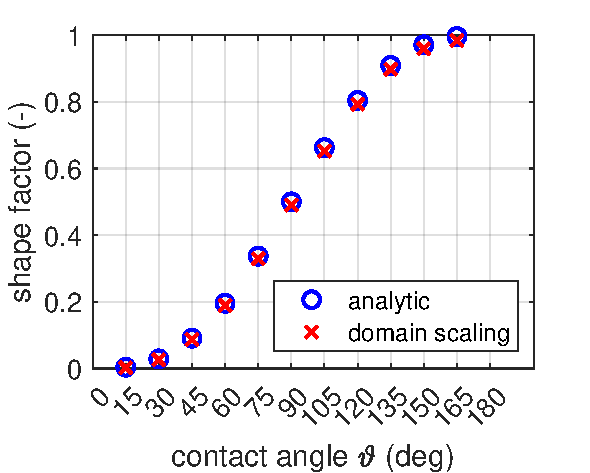
\includegraphics[width=0.49\textwidth]{NPA_PF_S_iso.pdf}};
		\draw node[inner sep =0] at (1.north west) {(a)};
		\draw node[inner sep =0] at (2.north west) {(b)};
	\end{tikzpicture}
	\caption{Results of the phase field simulation for determination of shape factor in heterogeneous nucleation with isotropic interface energy. In (a) the error in observed contact angles at the end of the simulation, in (b) the shape factor as obtained by domain scaling method.}
	\label{fig_result_NPA_PF_S_iso}
\end{figure}

Firstly, it is interesting that the observed contact angles $\vartheta_{obs}$ differed from those imposed by the boundary conditions $\vartheta$ significantly more than in the tilted line validation. This can be seen in the Figure~\ref{fig_result_NPA_PF_S_iso}a, where the difference $\vartheta_{obs}-\vartheta$ was plotted. The angle difference was larger than 5\textdegree~for 3 rather inclined angles (i.e. near 0\textdegree~or 180\textdegree). The deviation $\vartheta_{obs}-\vartheta$ did not depend on the phase field interface parameterization. In the base run, the interface width was $l_{IW}=$\qty{1e-9}{\m}, with 7 points through the interface. The compared simulations probed the effect of a) increasing the domain area, while keeping the $l_{IW}$ equal (effectively narrowing the physical interface width relative to the simulation initial condition) and of adding points to the interface (both actions refined the grid below the simulated initial condition) and both might improve phase field simulation accuracy in different regards. That did not happen in terms of the contact angles, though.

However, the shape factor determination was not affected heavily, because it turned out that there actually were very few points deviating from the expected circular shape and those were near the boundary. This is confirmed also by the obtained values of shape factor plotted in Figure~\ref{fig_result_NPA_PF_S_iso}, which follow closely the analytic prediction. The different interface parametrization yielded slight improvement in the shape factor values, but not relevant in the current application.

\subsection{Particle on a grain boundary (isotropic interface energy)}
%Here, the equilibrium stable shape is reached in a dynamic simulation. However, in the classical nucleation theory, it is in fact assumed that it stochastically appears due to local energy fluctuations in the nucleation spot. Among all the possible shapes with equal volume, those with lower total interface energy have higher nucleation probability. 
The present section investigates the theoretical case when the nucleus extends over the grain boundary and thus its wetting condition is unequal on the two sides. 

The geometry of the problem is sketched in~Figure~\ref{fig_sketch_particle_onGB}. When the two sides are wetted differently, it implies different contact angles and thus radii of the equilibrium shapes. That necessarily implies also different curvatures $K_{L/R}$. The chemical potential $\mu$ (the driving force, see~\eqref{eq_chempot_constant}) 
\begin{equation}
	\mu = \sigma K \,,
\end{equation}
over the whole stable shape must be a constant in order to have it in equilibrium. But for a constant $\sigma$ that cannot be achieved when there is a different curvature $K_{L/R}$ imposed on the left and right side.

Nevertheless, it is known that nucleation may happen on top of grain boundaries. Additionally, the nuclei in classical nucleation theory do not necessarily have the interface-energy minimizing shape, even though that one is the most likely. Hence, even if the shape is not in equilibrium, we assume that it could nucleate. Supposedly, it could survive by sliding to the lower-energy side of the grain boundary. Using the domain scaling procedure, the shape factor of the unknown compound shape can be quantified.

To reduce the simulation time, the initial condition was a shape combined from parts of the equilibrium shapes from both sides, connected by a tangent line to prevent dents in the initial shape (the initial condition was very similar to the problem sketch in Figure~\ref{fig_sketch_particle_onGB}, only with the tangent line). The initial condition can be seen in Figure~\ref{fig_PF_nuclbarrier_ISO_onGB_contours}, it is the one with steps (due to discretization in the simulation grid).
\begin{figure}
	\centering
	\begin{tikzpicture}[scale=2.7]
		\def\thl{120}
		\def\thr{-60}
		\tikzmath{ \RL = 0.4/sin(\thl) ; \RR = 0.7/sin(-\thr) ; }
		\path (-1,0) coordinate (al);
		\path (1,0) coordinate (ar);
		\path (0,0) coordinate (c);
		\path (0,-0.4) coordinate (cb);
		\path (-0.4,0) coordinate (cpl);
		\path (0.7,0) coordinate (cpr);

		\draw[very thick, blue] ($(cpl)+(0,-0.04)$) -- node[midway,below] {$\sigma_{GB}^L$} ($(c)+(0,-0.04)$);
		\draw[very thick, magenta] ($(cpr)+(0,-0.04)$) -- node[midway,below] {$\sigma_{GB}^R$} ($(c)+(0,-0.04)$);		
		\draw[very thick] (al) -| (cb) |- (ar);
		\draw (cpl) arc (\thl+90:90:\RL) node (toppoint) {};
		\draw[dashed] (toppoint) -- (c) ;
		\draw (cpr) arc (90+\thr:90:\RR);
		\draw[gray] (cpl) node[above right] {$\vartheta_L$} -- ++(\thl:0.5);
		\draw[gray] (cpr) node[above left] {$\vartheta_R$}-- ++(180+\thr:0.5);
		\draw[gray] ($(cpl)+(0.3,0)$) arc (0:\thl:0.3);
		\draw[gray] ($(cpr)+(-0.3,0)$) arc (180:180+\thr:0.3);
		\draw node[above] at (al) {$\sigma_{S}^L$};
		\draw node[above] at (ar) {$\sigma_{S}^R$};
		\draw (-1.2,-0.8) rectangle (1.2,0.8);
		
		\def\vshift{-0.3}
		\draw[stealth-stealth] ($(cpr)+(0,\vshift)$) -- node[midway,below] {$l_{GB}^R$} ($(c)+(0.02,\vshift)$);	
		\draw[stealth-stealth] ($(cpl)+(0,\vshift)$) -- node[midway,below] {$l_{GB}^L$} ($(c)+(-0.02,\vshift)$);	
		\draw[stealth-stealth] ($(cpl)+(0,-0.55)$) -- node[midway,below] {$l_{GB}$} ($(cpr)+(0,-0.55)$);	
	\end{tikzpicture}
	\caption{A particle on a grain boundary. The specific interface energies $\sigma_S^{L/R}$ belong to the substrate-solution interfaces and $\sigma_{GB}^{L/R}$ to the respective grain boundaries. The grain boundary lengths $l_{GB}^{L/R}$ and $l_{GB}$ are indicated.}
	\label{fig_sketch_particle_onGB}
\end{figure}

In the computation of the total grain boundary energy (meaning the energy of the substrate-particle interface), there will be two segments now, one on the left and one on the right side from the grain boundary (see Figure~\ref{fig_sketch_particle_onGB}). These have lengths $l_{GB}^{L}, l_{GB}^{R}$ and specific grain boundary energies $\sigma_{GB}^L=\sigma_{S}^L-\sigma_P\cos(\vartheta_L)$ and $\sigma_{GB}^R=\sigma_{S}^L-\sigma_P\cos(\vartheta_R)$. The symbols $\sigma_{S}^L,\sigma_{S}^R$ stand for the substrate surface energy on either side of the grain boundary and $\sigma_{P}$ is the particle-liquid interface energy. It turns out, that to express the total interface energy change (upon the insertion of the particle on top of the grain boundary) $\Delta G_\sigma$, it is sufficient to assume only $\sigma_P,\vartheta_L,\vartheta_R$, as can be seen below
\begin{align}
	\Delta G_\sigma &= F(\eta,\nabla\eta) + l_{GB}^{L}(\sigma_{GB}^L-\sigma_{S}^L) + l_{GB}^{R}(\sigma_{GB}^R-\sigma_{S}^R) \\
	&= F(\eta,\nabla\eta) - \sigma_P[l_{GB}^{L}\cos(\vartheta_L) + l_{GB}^{R}\cos(\vartheta_R)] \,.
\end{align}

The symbol $F(\eta,\nabla\eta)$ again stands for the total particle-parent phase interface energy. In the general case, the individual segments $l_{GB}^{L}, l_{GB}^{R}$ will have different length, depending on where the grain boundary is positioned below the particle. 

\begin{figure}
	\centering
	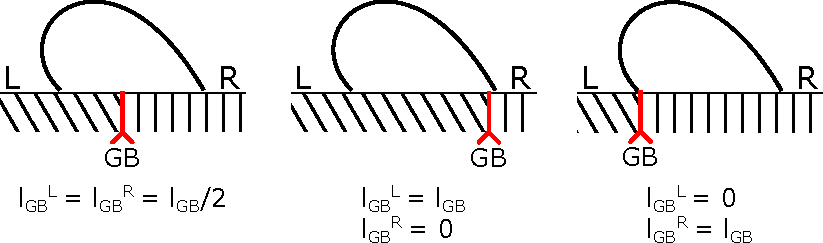
\includegraphics[width=\textwidth]{wulff_on_GB.pdf}
	\caption{Illustration of the three considered positions of grain boundary below the nucleus.}
	\label{fig_GB_below_wulff}
\end{figure}

Because the position of the grain boundary below the particle is chosen here, three shape factors were determined for each single shape, which corresponded to the cases when 
\begin{enumerate}
	\item $l_L = l_R = l_{GB}/2$, then $\Delta G_\sigma = F(\eta,\nabla\eta)- 0.5\sigma_Pl_{GB}[\cos(\vartheta_L)+\cos(\vartheta_R)]$
	\item $l_L = l_{GB}, l_R = 0$, then $\Delta G_\sigma = F(\eta,\nabla\eta)- \sigma_Pl_{GB}\cos(\vartheta_L)$,
	\item $l_L = 0, l_R = l_{GB}$, then $\Delta G_\sigma = F(\eta,\nabla\eta)- \sigma_Pl_{GB}\cos(\vartheta_R)$ and
\end{enumerate}
These cases were illustrated in Figure~\ref{fig_GB_below_wulff}. In the first case, the substrate grain boundary is just in the middle between the contact points. The second and third ones are limiting cases, when the contact point is infinitesimally just behind the substrate grains grain boundary, hence the full substrate-particle grain boundary lays on the either higher- or lower-energy grain. 

\alert{See Table~!!!! for details on the simulation} The contact angles $\vartheta_L,\vartheta_R$ were input to the simulation. In the presented results, it was assumed that $\vartheta_L=120$\textdegree and $\vartheta_R$ was varied between 30\textdegree-90\textdegree.

The first observation from the simulations is that the shape evolves, but even when it stops evolving, it moves as a block towards the side which has lower grain boundary energy. For the time evolution of the phase field contours in different cases see Figure~\ref{fig_PF_nuclbarrier_ISO_onGB_contours}. The intuitively correct direction of motion (i.e.e such which lowers the total grain boundary energy) is reproduced by the model, even though the system energy minimized in te phase field simulation does not account for the grain boundary explicitly. The reason is that the curvature driving force acts towards the center of curvature. As can be seen in Figure~\ref{fig_PF_nuclbarrier_ISO_onGB_contours}, the side with greater contact angle (and thus higher grain boundary energy) is more curved. The flatter is the opposite side, the less is the curvature driving force balanced. 

The velocity of the shape centroid in the x direction was obtained from linear fit through the x centroid coordinate in time, see Figure~\ref{fig_PF_nuclbarrier_ISO_onGB_results}a. The result quantifies the above reasoning, as it can be seen that lower $\vartheta_R$ (i.e. flatter right side) were associated with faster translation to the right.

The computed shape factors of the compound shapes were plotted in Figure~\ref{fig_PF_nuclbarrier_ISO_onGB_results}b with error bars indicating the possible span of values depending on the grain boundary position below the particle. The grain boundary energy contribution in the total energy of the particle seems to be a crucial factor for the nucleation probability. When the particle is sufficiently shifted to she lower-energy side, the deviation in shape may not cause dramatic increase in the nucleation barrier. In the opposite case (the particle is rather on the high-energy side), the nucleation can even be less likely than that of an isolated particle (homogeneous nucleation). In the extreme high-energy case for nearly all simulated $\vartheta_R$, the nucleation on top of the boundary was less likely than simply nucleating only on the high-energy part of the substrate. 

\begin{figure}
	\centering
	\begin{tikzpicture}
		\draw node[below right,inner sep=0] (lt) at (0,0) {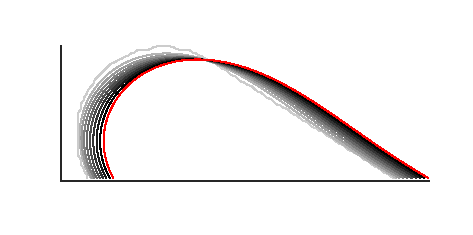
\includegraphics[width=0.48\textwidth]{PF_nuclbarr_ISO_onGB_contours_120x30.pdf}};
		\draw node[below right,inner sep=0] (rt) at (lt.north east) {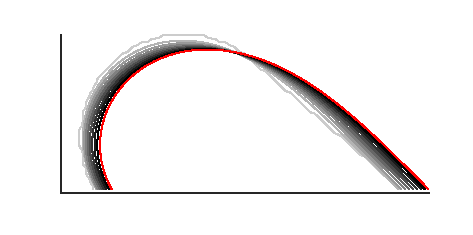
\includegraphics[width=0.48\textwidth]{PF_nuclbarr_ISO_onGB_contours_120x45.pdf}};
		\draw node[below right,inner sep=0] (lb) at (lt.south west) {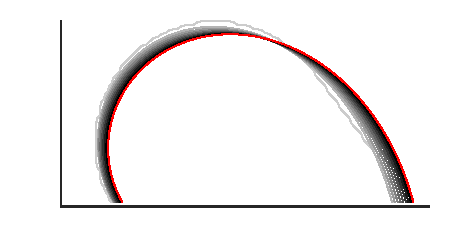
\includegraphics[width=0.48\textwidth]{PF_nuclbarr_ISO_onGB_contours_120x75.pdf}};
		\draw node[below right,inner sep=0] (rb) at (lb.north east) {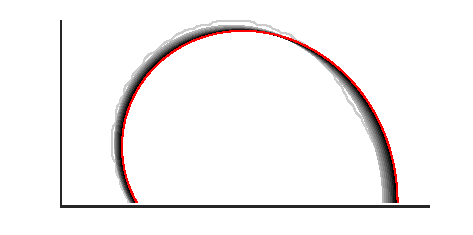
\includegraphics[width=0.48\textwidth]{PF_nuclbarr_ISO_onGB_contours_120x90.pdf}};
		
		\draw node[inner sep=0,right] at (lt.north west) {(a) $\vartheta_L=120$\textdegree, $\vartheta_R=-30$\textdegree};
		\draw node[inner sep=0,right] at (rt.north west) {(b) $\vartheta_L=120$\textdegree, $\vartheta_R=-45$\textdegree};
		\draw node[inner sep=0,right] at (lb.north west) {(c) $\vartheta_L=120$\textdegree, $\vartheta_R=-75$\textdegree};
		\draw node[inner sep=0,right] at (rb.north west) {(d) $\vartheta_L=120$\textdegree, $\vartheta_R=-90$\textdegree};
		
		\draw[-stealth,thick] ($(lt.center)+(-0.5,0) $) -- node[midway,below] {motion} ($(lt.center)+(0.5,0) $);
		\draw[-stealth,thick] ($(rt.center)+(-0.5,0) $) -- node[midway,below] {motion} ($(rt.center)+(0.5,0) $);
		\draw[-stealth,thick] ($(lb.center)+(-0.5,0) $) -- node[midway,below] {motion} ($(lb.center)+(0.5,0) $);
		\draw[-stealth,thick] ($(rb.center)+(-0.5,0) $) -- node[midway,below] {motion} ($(rb.center)+(0.5,0) $);
	\end{tikzpicture}
	\caption{Time evolution of phase field contours in the simulation of a particle on a grain boundary. The time evolves from gray to black contours, the last contour in the simulation is red.}
	\label{fig_PF_nuclbarrier_ISO_onGB_contours}
\end{figure}

\begin{figure}
	\centering
	\begin{tikzpicture}
		\draw node[below right,inner sep=0] (l) at (0,0) {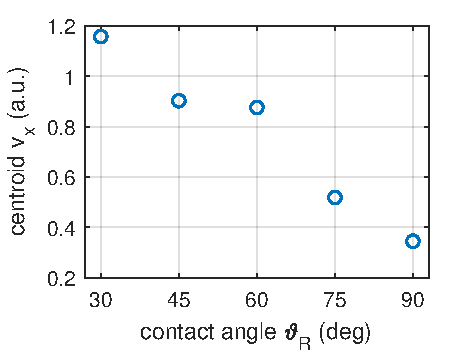
\includegraphics[width=0.48\textwidth]{PF_nuclbarr_ISO_onGB_centroidVx.pdf}};
		\draw node[below right,inner sep=0] (r) at (lt.north east) {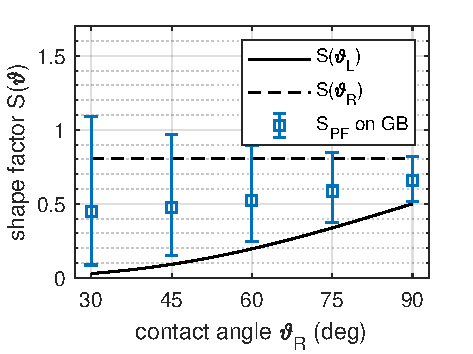
\includegraphics[width=0.48\textwidth]{PF_nuclbarr_ISO_onGB_SFrange.pdf}};
		\draw node[inner sep=0,right] at (l.north west) {(a) };
		\draw node[inner sep=0,right] at (r.north west) {(b)};
	\end{tikzpicture}
	\caption{Results from the simulation of a particle on a grain boundary. In (a) the x-direction velocity of the shape centroid as function of the right contact angle $\vartheta_R$ and in (b) the shape factor corresponding to the shape at the end of the simulation (i.e. red contours from Figure~\ref{fig_PF_nuclbarrier_ISO_onGB_contours}).}
	\label{fig_PF_nuclbarrier_ISO_onGB_results}
\end{figure}

\section{Summary and the author's contribution}
The author extended the multi-phase field model by Moelans~\cite{Moelans2008}. The work~\cite{Moelans2008} promoted usage of the model variant with constant interface width (here denoted IWc) with not-fully-variational formulation and described it in great detail.

At the beginning of the author's work, it was already known that IWc was not reliably reproducing the angles in triple junctions of interfaces with different interface energies~\cite{Moelans2010_thinfilm} (i.e. in pair-wise isotropic systems). The model variant with variable interface width and all anisotropy in the parameter $\gamma$ (here IWvG) was used in one grain growth study~\cite{Ravash2017}, but its better reliability in triple junction angles had not been documented yet.

As provided below with all details, the model extensions included
\begin{enumerate}
	\item Description of another model variant with all anisotropy in the parameter $\kappa$ and variable interface width (IWvK)
	\item Derivation of the governing equation for all the three model variants in both 2D and 3D for the case of inclination-dependent interface energy
	\item The model behavior depends heavily on proper parametrization of the equations. Best practices in parameters determination were  developed and described (different in each model variant) in order to assure control over both the local interface width and local interface energy. 
	\item In the IWvK model variant such boundary conditions were incorporated, which allowed to control the angle under which the interface intersecting the domain boundary will align.
\end{enumerate}

Besides the listed model extensions, the author also implemented two approaches adding the volume conservation to the system based on Allen-Cahn type of equations, namely one using Lagrange multipliers to conserve the volume and pne using fictitious concentration field. Volume conservation would be necessary in simulations, where the nucleus interacted dynamically with its surroundings, but these simulations were not needed eventually. Regardless, the model modifications including volume conservation were described in Appendix.

\section{TODO Conclusion}
 

%%%%%%%%%%%%%%%%%%%%%%%%%%%%%%%%%%%%%%%%%%%%%%%%%%
% Keep the following \cleardoublepage at the end of this file, 
% otherwise \includeonly includes empty pages.
\cleardoublepage

% vim: tw=70 nocindent expandtab foldmethod=marker foldmarker={{{}{,}{}}}
